\documentclass{article}
\usepackage[utf8]{inputenc}
\usepackage{amsfonts}
\usepackage{algorithm2e}
\usepackage{amsmath}
\usepackage[a4paper]{geometry}
\geometry{hscale=0.8,vscale=0.9,centering}
\usepackage{graphicx}
\usepackage{program}
\usepackage{ulem}
\usepackage{xcolor}
\usepackage{pdfpages}
\usepackage{hyperref}

\title{M1 Info – ARC - TD5}
\author{Olivier HUREAU - Groupe 3}
\date{25/03/2020}

\begin{document}
\maketitle

\section{Exercice 1}

\subsection{Assignements as three process}

We can transform the three assignements as three process such as :

Process P1 :

\begin{verbatim}
Process(A)
Begin
	Wait for 2 ns;
	S1 <= not A;
End process;
\end{verbatim}

Process P2 : 

\begin{verbatim}
Process(S1,B)
Begin
	Wait for 5 ns;
	S2 <= S1 nand B;
End process;
\end{verbatim}

Process P2 :

\begin{verbatim}
Process(S1, S2)
Begin
	Wait for 4 ns;
	SC <= S1 and S2;
End process;
\end{verbatim}

\subsection{Driver assignements}

\subsubsection{TC = 20 ns}
A is updated to '1', the process P1 is resumed and the drivers are updates as follow : 

\begin{verbatim}
S1 [ 1 / 22 ns | 
S2 [
SC [
\end{verbatim}
Next TC is 22 


\subsubsection{TC = 22 ns}

S1 is updated to '1', then the transaction is removes from the drive.

S1 is part of the sensitivity list of P2 and P3 so P2 and P3 are released and the drivers are updates as follow 

\begin{verbatim}
S1 [ 
S2 [ 0 / 27 ns |
SC [ 1 / 26 ns |
\end{verbatim}

Next TC is 26

\subsubsection{TC = 26 ns}

SC is updated to '1', then the transaction is removes from the drive.

SC is no part of a sensitivity list, no process resumes.

the drivers are updates as follow 

\begin{verbatim}
S1 [ 
S2 [ 0 / 27 ns |
SC [ 
\end{verbatim}

Next TC is 27

\subsubsection{TC = 27 ns}

S2 is updated to '0', then the transaction is removes from the drive.

S2 is  part of the sensitivity list of P3 so P3 resume 

the drivers are updates as follow 

\begin{verbatim}
S1 [ 
S2 [ 
SC [ 0 / 31 ns | 
\end{verbatim}

Next tc is 31

\subsubsection{TC = 31 ns}

SC is updated to '0', then the transaction is removes from the drive. SC is no part of a sensitivity list, no process resumes.

the drivers are updates as follow 

S1 [ 
S2 [ 
SC [

\subsubsection{All the drivers are empty }

There is a stabilization, we stop here


\section{Ecercice 2}
\subsection{}
The process equivalent to 
\begin{verbatim}
x <= 1 after 5 ns, 2 after 10 ns, 1 after 15 ns, 0 after 20 ns;
\end{verbatim}
is
 
\begin{verbatim}
Process
Begin
Wait for 5 ns;
x <= 1;
Wait for 5 ns;
x <= 5 ns;
Wait for 5 ns 
x <= 1;
Wait for 5 ns;
x <= 0;
Wait;
end process
\end{verbatim}

\subsection{}

The sensitivity list is empty there (the assignments do not depends of others signals). Moreover, we do not want the process to loop and execute only one times. 

Then the process does not resume.

\section{Exercice 3}

\subsection{Assignements as three process}

We can transform the three assignements as three process such as :

Process P1 :

\begin{verbatim}
Process(A, B)
Begin
	Wait for 3ns;
	X1 <= A or B;
End process;
\end{verbatim}

Process P2 : 

\begin{verbatim}
Process(X1)
Begin
	X2 <= not X1
End process;
\end{verbatim}

Process P3 :

\begin{verbatim}
Process(X2, C)
Begin
	Wait for 4 ns;
	Z <= X2 xor C;
End process;
\end{verbatim}

\subsubsection{TC = 22 ns}
A is updated to '0' and C is updated to '1'.
A is  part of the sensitivity list of P1 and C is part of the sensitivity list of P3. So P3 and P1 resumes.  

the drivers are updates as follow 

\begin{verbatim}
X1 [ 0 / 25 ns 
X2 [
Z  [ 1 / 26 ns
\end{verbatim}

Next TC is 25 

\subsubsection{TC = 25 ns}
X1 is updated to '0'. X1 is part of the sensitivity list of P2. So P2 resume.  


the drivers are updates as follow 

\begin{verbatim}
X1 [ 
X2 [ 1 / 25 ns
Z  [ 1 / 26 ns
\end{verbatim}

Next TC is 25 + delta 

\subsubsection{TC = 25 ns + delta}
X2 is updated to '1'. X2 is part of the sensitivity list of P3. So P3 resume.  

the drivers are updates as follow 

\begin{verbatim}
X1 [ 
X2 [ 
Z  [ 1 / 26 ns | 0 / 29 ns 
\end{verbatim}

Next TC is 26 ns

\subsubsection{TC = 26 ns}

Z is updated to '1', then the transaction is removes from the drive.

Z is no part of a sensitivity list, no process resumes.

the drivers are updates as follow 

\begin{verbatim}
X1 [ 
X2 [ 
Z  [ 0 / 29 ns 
\end{verbatim}

Next TC is 29

\subsubsection{TC = 29 ns}

Z is updated to '0', then the transaction is removes from the drive.

Z is no part of a sensitivity list, no process resumes.

the drivers are updates as follow 

\begin{verbatim}
X1 [ 
X2 [ 
Z  [ 
\end{verbatim}

Next TC is 29

\subsubsection{All the drivers are empty }

There is a stabilization, we stop here

\subsection{Results}

At 29 ns, we reach the following configuration (A = '0' , B = '0', C = '1' , Z = '0' , X1 = '0', X2 = '1')

\begin{figure}[!h]
\advance\leftskip+1cm
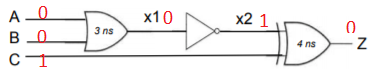
\includegraphics[scale=2]{Scheme.PNG}
\end{figure}

\newpage
\section{Exercise 4}

\subsection{Everytime a car wants to enter and the parking is not full, the input gate must open and must stay
open until the car has come in or the timeout is reached. }

We can rephrase as follow :
\begin{verbatim}
Everytime (
			- A car want to enter
			AND
			- The Parking is not full
		)
		
Then 

Untill ( 
		- !(Car Came out)
		OR
		- !(Timout reached)
		)
The gate are open
	
\end{verbatim}


\subsubsection{PSL Forumula}

\begin{verbatim}
Always ( 
(a car want to enter) and (parking is not full) 
=> Gate Open untill! ( (timeout is reached) or (the car as come in) )
) 
)
\end{verbatim}
\subsubsection{Give the corresponding PSL formula. Is it always satisfied? If not, enhance the formula to produce a version that is actually satisfied by this automaton}

It does not satisfied the automaton beacause it must not have a ticket insserted to go to state OPEN\_IN.

Then the formula to satisfied this automaton is :


\begin{verbatim}
Always ( 
(a car want to enter) and (parking is not full) and (no ticket is insserted) 
=> Gate Open untill! ( (timeout is reached) or (the car as come in) )
) 

)
\end{verbatim}



\subsection{Everytime a non-valid ticket is inserted, the output gate should not open }

\begin{verbatim}

Always ( the ticket is non valid => the output gate stay closed ) 


\end{verbatim}

 
\end{document}